\documentclass[12pt,a4paper]{article}

% ─── Page Layout ───────────────────────────────────────────────────────────────
\usepackage[a4paper, margin=0.8in, headheight=14pt]{geometry}

% ─── Fonts (XeLaTeX) ───────────────────────────────────────────────────────────
\usepackage{fontspec}
\usepackage{unicode-math}
\setmainfont{TeX Gyre Pagella}
\setmonofont[Scale=0.88]{TeX Gyre Cursor}
\setmathfont{Latin Modern Math}

% ─── Packages ──────────────────────────────────────────────────────────────────
\usepackage{xcolor}
\usepackage{colortbl}
\usepackage{titlesec}
\usepackage{enumitem}
\usepackage{tabularx}
\usepackage{longtable}
\usepackage{booktabs}
\usepackage{array}
\usepackage{amsmath}
\usepackage{tikz}
\usetikzlibrary{shapes.geometric, arrows.meta, positioning, calc, fit, decorations.pathreplacing, patterns}
\usepackage{tcolorbox}
\tcbuselibrary{skins, breakable}
\usepackage{hyperref}
\usepackage{fancyhdr}
\usepackage{graphicx}
\usepackage{microtype}
\hyphenpenalty=10000
\exhyphenpenalty=10000
\sloppy
\usepackage{caption}
\usepackage{setspace}
\usepackage{multirow}
\usepackage{tocloft}

% ─── Q&A helper ────────────────────────────────────────────────────────────────
\newcommand{\Q}[1]{\textbf{#1}\par\noindent\ignorespaces}

% ─── Colour Palette ────────────────────────────────────────────────────────────
\definecolor{myred}{RGB}{196,30,58}
\definecolor{mydark}{RGB}{30,30,50}
\definecolor{mygreen}{RGB}{14,120,80}
\definecolor{myteal}{RGB}{0,130,140}
\definecolor{myamber}{RGB}{180,100,0}
\definecolor{mypurple}{RGB}{100,30,160}
\definecolor{mygray}{RGB}{246,247,249}
\definecolor{mgframe}{RGB}{180,185,200}
\definecolor{watermark}{RGB}{145,150,170}
\definecolor{hdrred}{RGB}{250,232,235}
\definecolor{hdrgreen}{RGB}{220,244,233}
\definecolor{hdrteal}{RGB}{220,242,244}
\definecolor{hdramber}{RGB}{253,242,215}
\definecolor{hdrpurple}{RGB}{238,228,255}
\definecolor{hdrgray}{RGB}{238,240,245}

% ─── Section Formatting ────────────────────────────────────────────────────────
\titleformat{\section}
  {\large\bfseries\color{myred}}{\thesection.}{0.5em}{}
  [\vspace{1pt}{\color{myred}\rule{\linewidth}{0.8pt}}]
\titleformat{\subsection}
  {\normalsize\bfseries\color{myteal}}{\thesubsection}{0.5em}{}
\titlespacing*{\section}{0pt}{18pt}{7pt}
\titlespacing*{\subsection}{0pt}{11pt}{4pt}

% ─── Paragraph ─────────────────────────────────────────────────────────────────
\setlength{\parindent}{0pt}
\setlength{\parskip}{4pt}

% ─── TOC Styling ───────────────────────────────────────────────────────────────
\renewcommand{\cfttoctitlefont}{\large\bfseries\color{myred}}
\renewcommand{\cftaftertoctitle}{\par\noindent{\color{myred}\rule{\linewidth}{0.8pt}}}
\setlength{\cftbeforetoctitleskip}{0pt}
\setlength{\cftaftertoctitleskip}{6pt}
\renewcommand{\cftsecfont}{\normalsize\bfseries\color{mydark}}
\renewcommand{\cftsecpagefont}{\normalsize\bfseries\color{mydark}}
\renewcommand{\cftsecleader}{\cftdotfill{\cftdotsep}}
\setlength{\cftbeforesecskip}{7pt}
\renewcommand{\cftsubsecfont}{\small\color{mydark}}
\renewcommand{\cftsubsecpagefont}{\small\color{mydark}}
\setlength{\cftbeforesubsecskip}{3pt}
\setlength{\cftsubsecindent}{1.4em}

% ─── Table helpers ─────────────────────────────────────────────────────────────
\renewcommand{\arraystretch}{1.45}
\setlength{\tabcolsep}{6pt}
\arrayrulecolor{mydark}
\newcolumntype{B}[1]{>{\small\bfseries\raggedright\arraybackslash}m{#1}}
\newcolumntype{Y}{>{\small\raggedright\arraybackslash}X}
\renewcommand{\tabularxcolumn}[1]{m{#1}}

% ─── Header / Footer ───────────────────────────────────────────────────────────
\pagestyle{fancy}
\fancyhf{}
\fancyhead[L]{\small\color{myred}\textbf{ES-CS401}\;\color{mydark}--- Design and Analysis of Algorithms}
\fancyhead[R]{\small\color{myteal}\textbf{Module 3 Notes}}
\fancyfoot[C]{\small\color{mydark}\thepage}
\fancyfoot[R]{\small\color{watermark}\textit{\copyright\ Biraj Sarkar (CGEC)}}
\renewcommand{\headrulewidth}{0.5pt}
\renewcommand{\footrulewidth}{0.3pt}

% ─── Hyperref ──────────────────────────────────────────────────────────────────
\hypersetup{
  colorlinks=true, linkcolor=myteal, urlcolor=myteal,
  pdfauthor={Biraj Sarkar (CGEC)},
  pdftitle={ES-CS401 --- Module 3 Notes: Graph and Tree Algorithms}
}

% ─── tcolorbox styles ──────────────────────────────────────────────────────────
\tcbset{
  tikzbox/.style={
    colback=mygray, colframe=mgframe, boxrule=0.6pt, arc=4pt,
    left=8pt, right=8pt, top=6pt, bottom=6pt,
    colbacktitle=mgframe, coltitle=mydark, fonttitle=\small\bfseries
  },
  defbox/.style={
    colback=hdrgreen, colframe=mygreen, boxrule=0.8pt, arc=4pt,
    left=9pt, right=9pt, top=6pt, bottom=6pt,
    colbacktitle=mygreen, coltitle=white, fonttitle=\small\bfseries
  },
  formulabox/.style={
    colback=hdrteal, colframe=myteal, boxrule=0.8pt, arc=4pt,
    left=9pt, right=9pt, top=7pt, bottom=7pt,
    colbacktitle=myteal, coltitle=white, fonttitle=\small\bfseries
  },
  examplebox/.style={
    colback=hdramber, colframe=myamber, boxrule=0.8pt, arc=4pt,
    left=9pt, right=9pt, top=6pt, bottom=6pt,
    colbacktitle=myamber, coltitle=white, fonttitle=\small\bfseries
  },
  masonbox/.style={
    colback=hdrpurple, colframe=mypurple, boxrule=0.8pt, arc=4pt,
    left=9pt, right=9pt, top=6pt, bottom=6pt,
    colbacktitle=mypurple, coltitle=white, fonttitle=\small\bfseries
  },
  exambox/.style={
    colback=hdrpurple, colframe=mypurple, boxrule=1pt, arc=5pt,
    left=10pt, right=10pt, top=8pt, bottom=8pt,
    colbacktitle=mypurple, coltitle=white, fonttitle=\bfseries,
    breakable, title after break={\textbf{Frequently Asked / Viva Questions (contd.)}}
  }
}
\tcbset{breakable}
\tcbset{after={\par\color{black}}}

% ─── TikZ styles ───────────────────────────────────────────────────────────────
\tikzset{
  block/.style={rectangle, draw=myteal, fill=hdrteal,
    text width=2.4cm, align=center, minimum height=0.95cm,
    font=\small, rounded corners=3pt, line width=0.7pt},
  redblock/.style={rectangle, draw=myred, fill=hdrred,
    text width=2.4cm, align=center, minimum height=0.95cm,
    font=\small, rounded corners=3pt, line width=0.7pt},
  amberblock/.style={rectangle, draw=myamber, fill=hdramber,
    text width=2.4cm, align=center, minimum height=0.95cm,
    font=\small, rounded corners=3pt, line width=0.7pt},
  sumjunc/.style={circle, draw=myamber, fill=hdramber,
    minimum size=0.62cm, font=\small, line width=0.8pt},
  arrow/.style={-Stealth, thick, color=mydark},
  redarrow/.style={-Stealth, thick, color=myred},
  line/.style={thick, color=mydark}
}

\begin{document}

% ─── Title Page ───────────────────────────────────────────────────────────────
\begin{center}
  {\LARGE\bfseries\color{myred} ES-CS401 --- Design and Analysis of Algorithms}\\[5pt]
  {\normalsize\color{mydark} Semester IV \quad$\bullet$\quad 3L:0T:0P \quad$\bullet$\quad 3 Credits}\\[3pt]
  {\normalsize\color{myteal}\textbf{Module 3 Exam Notes: Graph and Tree Algorithms}}\\[3pt]
  {\small\color{mydark} CGEC \;$|$\; B.Tech ECE (2023--27) \;$|$\; \textit{Biraj Sarkar}}
\end{center}
\vspace{2pt}
\noindent{\color{myred}\rule{\linewidth}{1.5pt}}
\vspace{2pt}

\hypersetup{linkcolor=mydark}
\tableofcontents
\hypersetup{linkcolor=myteal}
\newpage

\section{Graph and Tree Algorithms}
\subsection{Graph representation and basic terminology}
\begin{tcolorbox}[defbox, title={Graph and tree}]
A graph $G=(V,E)$ has vertices and edges. An edge may have a direction, a weight, or both. A tree is a connected acyclic undirected graph. A forest is a collection of trees. Vertices of a rooted tree can be viewed as parents and children starting at a chosen root.
\end{tcolorbox}

\par\vspace{5pt}
\begingroup
\setlength{\extrarowheight}{1pt}
\noindent\begin{tabularx}{\linewidth}{|B{3.5cm}|Y|Y|}
\hline
\textbf{Representation} & \textbf{Space} & \textbf{Typical use} \\ \hline
Adjacency list & $\Theta(V+E)$ & Visit just the neighbours of each vertex. Efficient for sparse graphs. \\ \hline
Adjacency matrix & $\Theta(V^2)$ & Test a specific adjacency in $O(1)$ time. Scanning all neighbours of one vertex costs $\Theta(V)$. \\ \hline
Edge list & $\Theta(E)$ edge records, plus any vertex records. & Scan or sort all edges for algorithms such as Bellman--Ford and Kruskal. \\ \hline
\end{tabularx}\par
\endgroup
Here $V$ and $E$ in complexity expressions denote the numbers of vertices and edges. Weighted matrices need a separate marker for a missing edge so that weight zero can still represent a real edge.

\subsection{Breadth-first search}
\begin{tcolorbox}[defbox, title={Breadth-first search (BFS)}]
BFS explores all vertices at distance $d$ from the source before exploring vertices at distance $d+1$, where distance is the number of edges. A FIFO queue maintains this order.
\end{tcolorbox}

\begin{tcolorbox}[formulabox, title={BFS for unweighted shortest paths}]
\begin{verbatim}
BFS(G, s):
    set every distance to infinity and every parent to NIL
    distance[s] = 0
    enqueue s
    while the queue is not empty:
        u = dequeue()
        for each v in Adj[u]:
            if distance[v] is infinity:
                distance[v] = distance[u] + 1
                parent[v] = u
                enqueue v
    return distance, parent
\end{verbatim}
\end{tcolorbox}

\textbf{Correctness.} The first discovered path of length $d$ is valid by following parents. A shorter path would have a predecessor at an earlier level. BFS would have processed that predecessor and discovered the vertex earlier. Assign distance before enqueuing so each vertex enters the queue once. The full traversal costs $O(V+E)$ with adjacency lists and $O(V^2)$ with a matrix. Parents and the queue use $O(V)$ extra memory.

\subsection{Depth-first search and rooted tree traversals}
\begin{tcolorbox}[defbox, title={Depth-first search (DFS)}]
DFS follows a branch until no undiscovered successor remains, then returns to a previous decision. A recursive call stack or explicit stack represents the active path.
\end{tcolorbox}

\begin{tcolorbox}[formulabox, title={DFS with discovery and finishing times}]
\begin{verbatim}
DFS(G):
    mark all vertices WHITE
    clock = 0
    for each vertex u:
        if u is WHITE:
            Visit(u)

Visit(u):
    mark u GRAY and record discovery time with ++clock
    for each v in Adj[u]:
        if v is WHITE:
            parent[v] = u
            Visit(v)
        else if v is GRAY:
            record a back edge in a directed graph
    mark u BLACK and record finish time with ++clock
\end{verbatim}
\end{tcolorbox}

A DFS tree edge first discovers a vertex. In a directed graph a gray target lies on the active ancestor path, so a back edge proves a cycle. Edges to already finished vertices may be forward (to a descendant) or cross (between completed branches). In an undirected graph ignore the reverse copy of the parent tree edge when testing for cycles. A full DFS costs $O(V+E)$ time and $O(V)$ auxiliary space.
\begin{tcolorbox}[tikzbox, title={Directed graph for the traversal and ordering traces}]
\centering
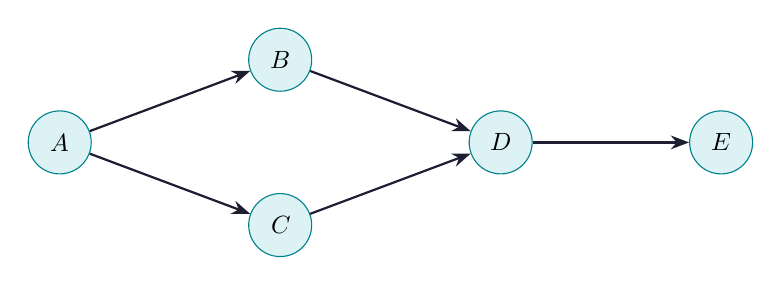
\begin{tikzpicture}[every node/.style={font=\small}]
\tikzset{vertex/.style={circle,draw=myteal,fill=hdrteal,minimum size=8mm,inner sep=0pt}}
\node[vertex] (a) at (0,0) {$A$};
\node[vertex] (b) at (2.8,1.05) {$B$};
\node[vertex] (c) at (2.8,-1.05) {$C$};
\node[vertex] (d) at (5.6,0) {$D$};
\node[vertex] (e) at (8.4,0) {$E$};
\draw[arrow] (a)--(b);
\draw[arrow] (a)--(c);
\draw[arrow] (b)--(d);
\draw[arrow] (c)--(d);
\draw[arrow] (d)--(e);
\end{tikzpicture}\par
\end{tcolorbox}

\begin{tcolorbox}[examplebox, title={BFS levels and DFS times}]
Assume alphabetical neighbour order and source $A$. BFS removes $A,B,C,D,E$ from its queue and records distances $0,1,1,2,3$. The parent of $D$ is $B$, since $B$ is processed before $C$. DFS visits $A,B,D,E$ first. After finishing that branch it visits $C$. The discovery/finish pairs are:
\[
A:(1,10),\quad B:(2,7),\quad C:(8,9),\quad D:(3,6),\quad E:(4,5).
\]
The edge $C\to D$ reaches a completed branch in this DFS.
\end{tcolorbox}

\par\vspace{5pt}
\begingroup
\setlength{\extrarowheight}{1pt}
\noindent\begin{tabularx}{\linewidth}{|B{3.4cm}|Y|Y|}
\hline
\textbf{Rooted tree visit} & \textbf{Order} & \textbf{Typical application} \\ \hline
Preorder & Root, then subtrees. & Copy a hierarchy or emit a prefix expression. \\ \hline
Inorder & Left subtree, root, right subtree in a binary tree. & Read a binary search tree in key order. \\ \hline
Postorder & Subtrees, then root. & Evaluate an expression tree or delete children before the parent. \\ \hline
Level order & Queue from the root, one layer at a time. & List nodes by depth. \\ \hline
\end{tabularx}\par
\endgroup

\section{Shortest Paths and Transitive Closure}
\subsection{Relaxation and Dijkstra's algorithm}
\begin{tcolorbox}[defbox, title={Shortest path and relaxation}]
A shortest path minimises the sum of edge weights between specified vertices. Relaxing an edge $u\to v$ replaces $d[v]$ by $d[u]+w(u,v)$ when that value is smaller, and records $u$ as the predecessor. An infinite label represents no path yet discovered.
\end{tcolorbox}

\begin{tcolorbox}[formulabox, title={Dijkstra with a min-priority queue}]
\begin{verbatim}
Dijkstra(G, s):
    initialise d[s] = 0 and all other distances to infinity
    keep unsettled vertices in a min-priority queue by d
    while the queue is not empty:
        u = extract-min()
        if d[u] is infinity: break
        for each edge u -> v with v unsettled:
            if d[u] + weight(u, v) < d[v]:
                update d[v] and parent[v]
                decrease the queue key of v
    return d, parent
\end{verbatim}
\end{tcolorbox}

\textbf{Why the extracted distance is final.} On any hypothetical shorter path to the extracted vertex, consider the first unsettled vertex. Its settled predecessor would already have relaxed the edge into it. With nonnegative edge weights, the prefix up to that first unsettled vertex costs no more than the shorter path. Its queue key would therefore be smaller than the extracted key, a contradiction.
\begin{tcolorbox}[examplebox, title={Dijkstra trace}]
Use the directed weighted edges $A\to B:4$, $A\to C:1$, $C\to B:2$, $C\to D:5$ and $B\to D:1$. Starting at $A$, settle in this order:
\par\vspace{5pt}
\begingroup
\setlength{\extrarowheight}{1pt}
\noindent\begin{tabularx}{\linewidth}{|B{2.4cm}|Y|Y|Y|}
\hline
\textbf{Settled vertex} & \textbf{$d[B]$} & \textbf{$d[C]$} & \textbf{$d[D]$} \\ \hline
$A$ & $4$ & $1$ & $\infty$ \\ \hline
$C$ & $3$ & $1$ & $6$ \\ \hline
$B$ & $3$ & $1$ & $4$ \\ \hline
$D$ & $3$ & $1$ & $4$ \\ \hline
\end{tabularx}\par
\endgroup
Predecessors recover $A\to C\to B\to D$ of cost $4$. A binary heap gives $O((V+E)\log V)$ time. An array-based minimum scan gives $O(V^2)$ when using an adjacency matrix.
\end{tcolorbox}

\begin{tcolorbox}[masonbox, title={Dijkstra requires nonnegative weights}]
Take $s\to u:2$, $s\to v:5$, $v\to u:-4$. Finalising $u$ at value $2$ misses the better route of cost $1$. The graph does not need a negative cycle for Dijkstra to fail.
\end{tcolorbox}

\subsection{Bellman--Ford and negative cycles}
\begin{enumerate}[leftmargin=*, itemsep=3pt, topsep=4pt]
  \item Set $d[s]=0$ and every other value to infinity.
  \item Repeat up to $V-1$ full passes over all edges, relaxing from finite labels. Stop early if a pass makes no change.
  \item Scan all edges once more. A further improvement from a finite label signals a reachable negative-weight cycle. Such a cycle makes finite minimum walk costs undefined for vertices reachable from it.
\end{enumerate}
\textbf{Proof outline.} Any finite label is the length of a concrete walk. After $k$ complete passes, each walk using at most $k$ edges has had a chance to improve its final label. When no reachable negative cycle is relevant, a shortest path can be chosen simple and uses at most $V-1$ edges. If a reachable negative cycle exists and every edge on it satisfies the no-improvement inequalities, summing those inequalities around the cycle contradicts its negative total weight. Worst-case time is $O(VE)$ for edge scans plus $O(V)$ initialisation.
\begin{tcolorbox}[examplebox, title={A negative edge that Bellman--Ford handles}]
Take $s\to A:4$, $s\to B:5$, $A\to B:-2$, $B\to C:3$, $A\to C:4$. In that edge order, the first pass sets $A=4$, improves $B$ from $5$ to $2$, and sets $C=5$. The result stays unchanged in the next pass. The shortest route to $C$ is $s,A,B,C$, using the negative edge once.
\end{tcolorbox}

For a DAG, process vertices in topological order and relax outgoing edges once. This takes $O(V+E)$ time and supports negative weights because cycles are absent.

\subsection{Floyd--Warshall and Warshall}
\begin{tcolorbox}[defbox, title={Transitive closure}]
The transitive closure records which ordered pairs have a directed path. In a \textbf{reflexive} closure, also include paths of length zero, so every diagonal entry is true.
\end{tcolorbox}

\begin{tcolorbox}[formulabox, title={Two forms of the intermediate-vertex recurrence}]
Order the vertices $1,\dots,V$. At stage $k$ determine whether the best route from $i$ to $j$ can use vertex $k$ in addition to earlier intermediate vertices.
\begin{align*}
D^{(k)}_{ij}
 &=\min\{D^{(k-1)}_{ij},D^{(k-1)}_{ik}+D^{(k-1)}_{kj}\},\\
R^{(k)}_{ij}
 &=R^{(k-1)}_{ij}\lor
   (R^{(k-1)}_{ik}\land R^{(k-1)}_{kj}).
\end{align*}
Use Floyd--Warshall for distance and Warshall for Boolean reachability. Start distances with edge weights, zero on the diagonal in the absence of negative self-loops, and infinity for missing edges. If self-loops are present, initialise each diagonal to the minimum of zero and its loop weight. Start Boolean entries with adjacency and choose the diagonal convention. In either algorithm $k$ is the outer loop. Time is $O(V^3)$ and in-place memory for the matrix is $O(V^2)$.
\end{tcolorbox}

\begin{tcolorbox}[examplebox, title={Intermediate vertex update}]
If $A\to B$ has cost $4$, $B\to C$ cost $2$ and $A\to C$ cost $9$, the stage allowing $B$ improves $D[A,C]$ to $6$. In a Boolean graph with just $A\to B$ and $B\to C$, that same stage sets $R[A,C]$ to true despite no direct edge. A negative diagonal after Floyd--Warshall indicates a negative cycle.
\end{tcolorbox}

\section{Spanning Trees and Topological Ordering}
A minimum spanning tree minimises wiring cost when edges are weighted. A topological order handles a different task: scheduling directed dependencies.
\subsection{Minimum spanning tree and the cut property}
\begin{tcolorbox}[defbox, title={Minimum spanning tree}]
An MST is a spanning tree of minimum total edge weight in a connected undirected weighted graph. It has $V-1$ edges and connects every vertex. A disconnected graph has a minimum spanning forest. The objective is total wiring cost, while a shortest-path tree minimises distances from one source.
\end{tcolorbox}

\textbf{Exchange proof for a safe edge.} A cut partitions the vertices into two sets. Assume the current chosen edges belong to some MST and none crosses this cut. Let $e$ be a minimum-weight crossing edge. If an MST containing the chosen edges omits $e$, adding $e$ forms a cycle containing another crossing edge $f$. Remove $f$. It was not among the chosen edges. Since $w(e)\le w(f)$, the result is also an MST and includes $e$.
\par\vspace{5pt}
\begingroup
\setlength{\extrarowheight}{1pt}
\noindent\begin{tabularx}{\linewidth}{|B{3.0cm}|Y|Y|}
\hline
\textbf{Algorithm} & \textbf{Greedy rule} & \textbf{Cost with common structures} \\ \hline
Kruskal & Sort edges by weight. Accept an edge only when its endpoints belong to different components. & $O(E\log E)$ plus near-linear disjoint-set operations. \\ \hline
Prim & Grow one tree from a start. Add a cheapest edge from the current tree to an outside vertex. & $O((V+E)\log V)$ with a binary heap and adjacency lists. \\ \hline
\end{tabularx}\par
\endgroup
\textbf{Implementation.} In Kruskal, start with one disjoint set per vertex. For each edge in increasing weight order, compare its two set representatives. If they differ, choose the edge and union the sets. In Prim, store each outside vertex's cheapest edge into the current tree. Extract the vertex with minimum key, add its stored edge, and update the keys of its outside neighbours.

\begin{tcolorbox}[examplebox, title={Kruskal and Prim on the same network}]
Let $AB=1$, $BC=2$, $AC=3$, $CD=4$, $BD=5$, $AD=7$. Kruskal accepts $AB$ and $BC$, rejects $AC$ because $A$ and $C$ are already connected, and accepts $CD$. Prim from $D$ takes $DC$ (4), $CB$ (2), then $BA$ (1). Both have cost $7$. Equal-weight edges can give several valid MSTs. Negative edge weights are permitted.
\end{tcolorbox}

\subsection{Topological sorting of a DAG}
\begin{tcolorbox}[defbox, title={Topological order}]
A topological ordering of a directed graph lists every vertex so that each edge $u\to v$ places $u$ before $v$. Such an order exists exactly for a directed acyclic graph (DAG).
\end{tcolorbox}

\begin{tcolorbox}[formulabox, title={Kahn's indegree algorithm}]
\begin{verbatim}
Compute indegree of every vertex.
Enqueue every vertex whose indegree is zero.
While the queue is nonempty:
    remove u and append it to the order
    for each edge u -> v:
        decrement indegree[v]
        if indegree[v] becomes zero:
            enqueue v
If the order has fewer than V vertices, report a cycle.
\end{verbatim}
\end{tcolorbox}

Every removed vertex has no remaining incoming edge. If no vertex can be removed while vertices remain, repeatedly following incoming edges in that finite remainder reaches a cycle. DFS offers another method: reject back edges and output vertices in decreasing finish time. In the traversal example the DFS order is $A,C,B,D,E$. Both methods run in $O(V+E)$ time. Tasks with no dependency between them may appear in either order.

\section{Network Flow Algorithms}
\subsection{Flow, cuts and the residual graph}
\begin{tcolorbox}[defbox, title={Feasible flow}]
A directed network gives each edge a capacity $c(u,v)\ge0$, with source $s$ and sink $t$. A feasible flow satisfies $0\le f(u,v)\le c(u,v)$ and conserves flow at intermediate vertices. The value $|f|$ is the net flow leaving $s$. An $s$--$t$ cut partitions vertices into $S$ and its complement. The cut capacity sums only original edges from $S$ to the complement.
\end{tcolorbox}

The residual graph contains unused forward capacity and reverse arcs that allow a previous allocation to be reduced. For a single original edge, the forward residual is $c-f$ and the reverse residual is $f$. When both directions were originally present, keep their edge contributions distinct or combine them consistently.
\begin{tcolorbox}[formulabox, title={Ford--Fulkerson and Edmonds--Karp}]
\begin{verbatim}
Start with zero flow.
While the residual graph has a path from s to t:
    find the minimum residual capacity on the path
    augment by this bottleneck amount
    update forward and reverse residual capacities
Return the final flow.
For Edmonds--Karp, find each residual path with BFS.
\end{verbatim}
\end{tcolorbox}

\textbf{Max-flow min-cut argument.} Conservation implies that every flow's value is at most any cut capacity. If no augmenting path remains, let $S$ be the residually reachable set from $s$. Every original arc from $S$ to the other side is saturated and any original arc in the reverse direction carries zero. Hence the flow equals the capacity of this cut and is maximum.
\begin{tcolorbox}[tikzbox, title={Flow network for the augmenting-path trace}]
\centering
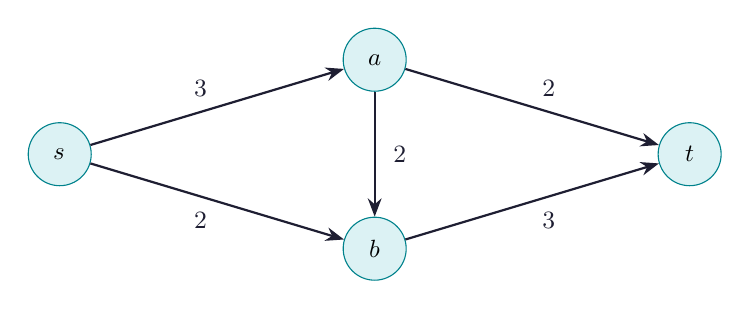
\begin{tikzpicture}[every node/.style={font=\small}]
\tikzset{vertex/.style={circle,draw=myteal,fill=hdrteal,minimum size=8mm,inner sep=0pt}}
\node[vertex] (s) at (0,0) {$s$};
\node[vertex] (a) at (4,1.2) {$a$};
\node[vertex] (b) at (4,-1.2) {$b$};
\node[vertex] (t) at (8,0) {$t$};
\draw[arrow] (s)--node[above left] {3} (a);
\draw[arrow] (s)--node[below left] {2} (b);
\draw[arrow] (a)--node[right=3pt] {2} (b);
\draw[arrow] (a)--node[above right] {2} (t);
\draw[arrow] (b)--node[below right] {3} (t);
\end{tikzpicture}\par
\end{tcolorbox}

\begin{tcolorbox}[examplebox, title={Augmenting paths with cancellation}]
\par\vspace{5pt}
\begingroup
\setlength{\extrarowheight}{1pt}
\noindent\begin{tabularx}{\linewidth}{|B{3.45cm}|Y|Y|}
\hline
\textbf{Residual path} & \textbf{Bottleneck} & \textbf{Flow value afterwards} \\ \hline
$s,a,b,t$ & 2 & 2 \\ \hline
$s,a,t$ & 1 & 3 \\ \hline
$s,b,t$ & 1 & 4 \\ \hline
$s,b,a,t$ & 1 & 5 \\ \hline
\end{tabularx}\par
\endgroup
The last path uses the residual reverse arc $b\to a$, reducing the original flow on $a\to b$ from 2 to 1. The cut $S=\{s\}$ has capacity $3+2=5$. The exhibited feasible flow reaches this upper bound.
\end{tcolorbox}

With integral capacities, Ford--Fulkerson has at most $|f^*|$ augmentations from zero because each increases the value by at least one. With $O(V+E)$ residual searches the total is $O((V+E)|f^*|)$ plus initialisation. This bound depends on capacity magnitude. Edmonds--Karp uses shortest residual paths in number of edges and has the polynomial bound $O(VE^2)$ after isolated vertices are discarded. Uses include matching, bandwidth allocation and project selection.

\subsection{Application: matching as unit-capacity network flow}
A \textbf{matching} is a set of edges sharing no endpoints. To match workers on the left to compatible jobs on the right, add edges of capacity 1 from the source to each worker, from workers to compatible jobs, and from each job to the sink.
\begin{itemize}[leftmargin=*, itemsep=3pt]
  \item A matching of size $k$ creates a flow of value $k$ by sending one unit along each selected worker--job path.
  \item Integral flow cannot use a worker or a job twice because its edge to the source or sink has capacity 1. Read edges carrying one unit to obtain the matching.
  \item Starting from zero and augmenting integral capacities preserves integrality. Max flow therefore returns a maximum-cardinality matching.
\end{itemize}
\begin{tcolorbox}[examplebox, title={Why rerouting beats an early assignment}]
Worker $A$ can do jobs $X$ and $Y$. Worker $B$ can do only $X$. If the first augmenting path assigns $A$ to $X$, use the next residual path $s\to B\to X\to A\to Y\to t$. The reverse arc $X\to A$ cancels $A$'s old assignment. The new matching uses $B$--$X$ and $A$--$Y$. The two source arcs give capacity 2, so the matching is maximum.
\end{tcolorbox}

\newpage
\begin{center}
  {\large\bfseries\color{myred} Quick Revision --- Module 3}\\[3pt]
  {\small\color{mydark} Graph and Tree Algorithms $|$ ES-CS401}
\end{center}
\noindent{\color{myred}\rule{\linewidth}{1.2pt}}\par\vspace{4pt}

\begin{tcolorbox}[formulabox, title={Key Concepts at a Glance}]
\renewcommand{\arraystretch}{1.35}
\noindent\begin{tabularx}{\linewidth}{B{4.5cm}Y}
BFS and DFS & $O(V+E)$ with adjacency lists, $O(V)$ auxiliary memory. \\[3pt]
Shortest paths & Dijkstra for nonnegative edges. Bellman--Ford for negative edges. DAGs permit one topological pass. \\[3pt]
All-pairs and closure & Floyd--Warshall (min plus) and Warshall (Boolean), both $O(V^3)$. \\[3pt]
Residual capacity & Unused forward capacity and reversible past flow. \\[3pt]
Optimal flow certificate & A feasible flow and cut with matching value and capacity. \\[3pt]
\end{tabularx}\par
\end{tcolorbox}

\begin{tcolorbox}[defbox, title={One-Line Definitions}]
\begin{itemize}[leftmargin=*, itemsep=3pt, topsep=4pt]
  \item \textbf{Tree.} A connected undirected graph with no cycle.
  \item \textbf{Relaxation.} Improve the known distance by trying one additional edge.
  \item \textbf{Cut.} A partition of the vertices into two sets.
  \item \textbf{Augmenting path.} A source-to-sink path using positive residual capacities.
\end{itemize}
\end{tcolorbox}

\begin{tcolorbox}[exambox, title={Frequently Asked / Viva Questions}]
\begin{enumerate}[topsep=0pt, label=\textbf{Q\arabic*.}, itemsep=5pt, leftmargin=*]
  \item \Q{Why does BFS use FIFO?}
    The queue processes all vertices of one distance before the next layer.
  \item \Q{Which DFS edge certifies a directed cycle?}
    An edge to a gray ancestor on the active path.
  \item \Q{How is a path reconstructed?}
    Follow predecessors from target to source and reverse the resulting list.
  \item \Q{What breaks Dijkstra?}
    A negative edge can later improve a previously settled label.
  \item \Q{When can Bellman--Ford report a negative cycle?}
    A finite-label relaxation is still possible after the usual passes.
  \item \Q{What is the outer loop in Warshall?}
    The intermediate vertex index.
  \item \Q{Which structure supports Kruskal?}
    Disjoint-set union detects whether endpoints already share a component.
  \item \Q{How many edges are in a spanning tree?}
    $V-1$ for a connected graph with $V$ vertices.
  \item \Q{What happens if Kahn's queue empties early?}
    The remaining directed graph contains a cycle.
  \item \Q{Why include residual reverse arcs?}
    They permit cancellation and rerouting of earlier flow choices.
  \item \Q{How does Edmonds--Karp select paths?}
    It uses BFS to select a path with the fewest residual edges.
\end{enumerate}
\end{tcolorbox}

\begin{tcolorbox}[tikzbox, title={Summary Comparison}]
\par\vspace{5pt}
\begingroup
\setlength{\extrarowheight}{1pt}
\noindent\begin{tabularx}{\linewidth}{|B{3.45cm}|Y|Y|}
\hline
\textbf{Task} & \textbf{Algorithm} & \textbf{Key condition} \\ \hline
Minimum edge count & BFS & Unweighted or uniform unit edge cost. \\ \hline
Minimum total wiring & Prim or Kruskal & Undirected weighted graph. \\ \hline
Prerequisite ordering & Kahn or DFS & Directed acyclic graph. \\ \hline
Maximum throughput & Edmonds--Karp & Nonnegative capacities with a source and sink. \\ \hline
\end{tabularx}\par
\endgroup
\end{tcolorbox}

\end{document}
